% !TEX root = ..\main.tex
\chapter{State-of-the-Art}
This chapter presentes topics which are relevant to this project. Section 2.1 looks into technical debt with its definitions, types etc. Section 2.2 looks into embedded systems and some of the challenges with it. Section 2.3 presents 


\section{Technical Debt}
The concept of technical debt was first introduced by Ward Cunningham in 1992 to communicate the problem with non-technical stakeholders\cite{p29-cunningham}. The concept was used to describe the system design trade-offs that are made everyday. To deliver business functionality as quickly as possible, \textit{'quick and dirty'} decisions leading to technical debt had to be made, which affect future development activities. Cunningham further describes technical debt as \textit{"shipping first time code is like going into debt. A little debt speeds development as long as it is paid back promptly with a rewrite"}. As time goes, technical debt accumulates interest leading to increased costs of a software system\cite{p31-guo,p35-klinger}. However, not all debts are necessarily bad. A small portion of debt might help developers speed up the development process in the short-term\cite{p31-guo}. 


%% The costs of technical debt
\begin{figure}[ht!]
	\centering
	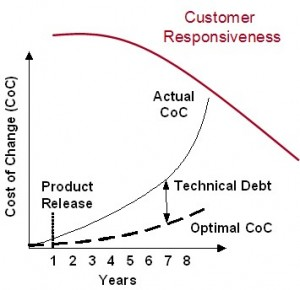
\includegraphics[width=0.8\textwidth]{images/techdebtCurve.jpg}
	\caption{The Technical Debt Curve\cite{jim-highsmith}}
	\label{fig:techDebtCurve}
\end{figure}

Figure \ref{fig:techDebtCurve} illustrates what happens as technical debt grows over time within a software product. Once we are on the far right of the curve, all choices are hard. The software controls us more than we control it.

%%%

\subsection{Definitions of Technical Debt}
McConnell describes TD as: \textit{a design or construction approach that is expedient in the short term but that creates a technical context in which the same work will cost more to do later than it would cost to do now (including the increased cost over time)}. He further splits the term into two categories based on how they are incurred, intentionally or unintentionally\cite{url-mcconnell}. The unintentional category includes debt that comes from doing a poor job. For example, uninntentional debt might be when a junior software developer writes bad code due to lack of knowledge and experience. Intentional debt occurs when an organization makes a decision to optimize for the present rather than the future. An example is when the project release must be done on time, or else there will not be a next release. This leads to bad decisions, like taking a shortcut to solve a problem, and then reconcile the problem after shipment

Fowlers presents a more formal explanation of how technical debt can occur\cite{url-fowler}. He categories technical debt into a quadrant with two dimensions, which he calls the \textit{"Technical Debt Quadrant"}. As seen in the Figure \ref{fig:techDebtQuad}, the debt is grouped into four categories: 

\begin{figure}[ht!]
	\centering
	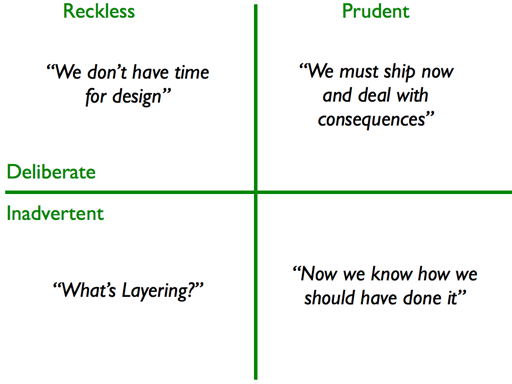
\includegraphics[width=0.8\textwidth]{images/techDebtQuadrant.png}
	\caption{Technical Debt Quadrant}
	\label{fig:techDebtQuad}
\end{figure}

\begin{itemize}
	\item \textbf{Reckless/Deliberate debt}: The team feels time pressure, and takes shortcuts intentionally without any thoughts on how to address the consequences in the future.
	\item \textbf{Reckless/Inadvertent debt}: Best practices when it comes to code and design is ignored, and a big mess in the codebase is made.
	\item \textbf{Prudent/Deliberate debt}: : The value of taking shortcuts is worth the cost of incurring debt in order to meet a deadline. The team is aware of the consequences, and has a plan in place to address them in the future. 
	\item \textbf{Prudent/Inadvertent debt}: Software development process is as much learning as it is coding. The team can deliver a valuable software with clean code, but in the end they might realize that the design could have been better.
\end{itemize}

Krutchen divides technical debt into two categories\cite{krutchen}. Visible debt that is visible for everyone. It containts elements such as new functionality to add and defects to fix. Invisible is the other category, debt that is only visible to software developers. Figure \ref{fig:techDebtLandscape} shows a map of the "technical debt landscape" which helps us to distinguish visible and invisible elements. On the left side of Figure \ref{fig:techDebtLandscape}, TD mostly affects the evolvability of the software system, while on the right it mainly affects maintainability.

\begin{figure}[ht!]
	\centering
	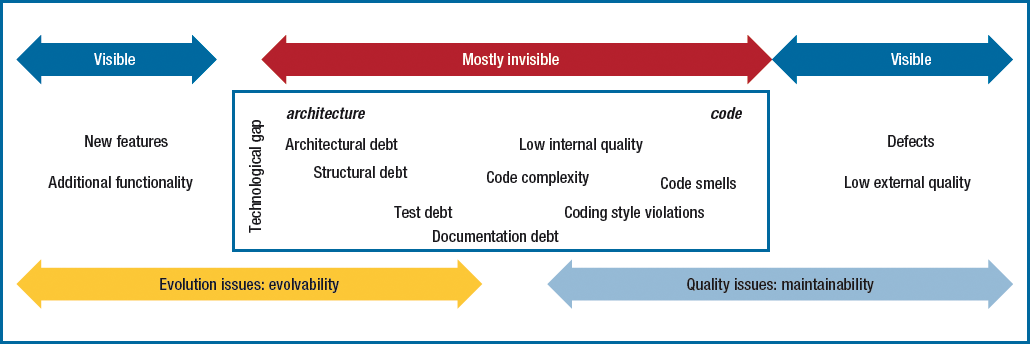
\includegraphics[width=1.0\textwidth]{images/techDebtLandscape.png}
	\caption{Technical Debt Landscaape}
	\label{fig:techDebtLandscape}
\end{figure}

\subsection{Comparison with financial debt}
Technical debt has many similarities to financial debt\cite{p50-allman,Zazworka:2011:PDD:1985362.1985372}:
\begin{itemize}
	\item You take a loan that has to be repaid later
	\item You usually repay the loan with interest
	\item If you can not pay back, a very high cost will follow. For example, you can loose your house or car.
\end{itemize}

Like financial debt, technical debt accrues interest over time which comes in the form of extra effort that has to be dedicated in future development because of bad choices\cite{p31-guo,p35-klinger}. Stakeholders can choose to continue paying the interest, or you can pay down the debt by refactoring the code or system into something better which reduces interest payments in the future\cite{url-fowler}. If the debt is not repaid, development might slow down, e.g, due to poor maintainability of the code. This can lead to software project failure and you might go bankrupt\cite{p50-allman}. There are some differences between financial and technical debt as well. The debt has to be repaid eventually, but not on any fixed schedule\cite{p50-allman}. This means that some debts may never have to be paid back, which depends on the interest and the cost of paying back the debt\cite{foser076-brown}. Example on interests can be be lower pace of development, low competitiveness, security flaws on the system, loss of developers and their expertise, poor internal collaboration environment, dissatisfied customers, and loss of market share\cite{p50-allman}.


\subsection{Causes and effects of technical debt}
Multiple studies have tried to analyze the reason for companies to incur technical debt.

%While financial debt occus from deliberate actions of taking a loan, technical debt may be caused by several factors. Antares categories these factors into four groups:
%\begin{itemize}
%	\item Work processes: Software development methology, can some tasks be automized (with a deploy script), is tests written after bug fixing, do you map and document shortcuts you take, is there any plans for techincal debt management later, is it important to implement new functionality or to make sure that the existing ones work propertly?
%	\item People (knowledge and capacity): Do you need some individuals to finish a task, Do you have the right people for the job, is enough training given to new people, what happens if you need someone who's on vacation/change project/is sick or something. You should keep this in mind and make a plan on how knowledge is transferred. Techcnical debt can be the reason for poor motivation and productivity which causes you to work poorly. 
%	\item Technology: Is solutions hard to integrate with other solutions, is all the systems out there compatible with newer technology, is there any outdated or duplicated code in the system, is all the systems secure, is the solutions old, or user friendly, is there some code which is hard to maintencance. 
%	\item Collaboration in the organization: Commuinication between developers and requirement people. You often get a list with requirements, is the list understandable? Do we work with a backlog with tasks that should have been solved long time ago, but not which is not "actual" now?
%\end{itemize}
%Developers might not care about the product because they don't feel that they "own" what's being made. They get told what do to, but not more than that. Can't make requirements.


%Operating technical debt might be to maintenance and manage existing code rather than implementing new functionality. It is important to keep track of the technical debt, and incur interest payments, before it makes troubles for you. Do do that, you could for example set up a plan for repayment which tells you something about how the debt shall be repayed. Scrum can be used to do this for example, where you split the repayment plan to smaller parts where you estimate and prioritize tasks. It is important to remember that taking too much loan might cause problems. As mentioned ealier, technical debt can be seen as taking a financial loan according to Cunningham. The loan has to be repaid with interests. Technical debt uses time and effort as repayment. It is acceptable to take a loan, but it should be controlled. Do not take loan than what you are able to handle. Think with your head.

%Main developers behind a software project aren't the one who usually maintain the code. Companies often has policies where they transfer a project to new developers after the development phase is over. The reasons could be to save money, or that the new developers might work more. These maintenance people often haas to repay the debt. The main developers gets awarded for their implementation speed rather than thinking on maintanence and evolution. They can often be placed on new projects before the debt has to be paid back, making them unavaiable for a period. Too few systems also has TODO or FIXME comments in their source code.

Klinger et al.\cite{p35-klinger} carried out an industrial case study at IBM where four technical architects with different backgrounds were interviewed. The goal was to examine how the decisions to incur debt were taken, and the extent to which the debt provided leverage\cite{p35-klinger}. The study revealed that the company failed to assess the impact of intentionally incurring debt on projects. Decisions regarding technical debt were rarely quantified. The study also revealed big organizational gaps among the business, operational, and technical stakeholders, which incurred debt. When the project team felt pressure from the stakeholders, technical debt decisions were made without quantifications of possible impacts.

Lim et al.\cite{lim-taksande} show that technical debt is not always the result of poor developer disciplines, or sloppy programming. It can also include intentionals decisisions to trade off competing concerns during business pressure. They also found out that technical debt can be used in short term to capture market share and to collect customers feedback early. In the long term, techical debt tended to be negative. These tradeoffs included increased complexity, reduced performance, low maintainability, and fragile code. This led to bad customer satisfaction and extra working hours. In come cases, the short term benefits of technical debt outweighted the future costs.

Guo et al.\cite{guo2011tracking} studied the effects of technical debt by tracking a single delayed maintenance task in a real software project throughout its lifecycle, and simulated how managing technical debt can impact the project result. The results showed that delaying the maintenance task would have almost tripled the costs, if it had been done later.

Siebra et al.\cite{p247-siebra} carried out an industrial case study where they analyzed documents, emails code files, and had interviews with developers and project managers. This case lasted for six years. This study revealed that technical debt were mainly taken by strategic decisions. They also found out that using a unique specialist could lead the development team to solutions that the specialist wanted and believe were correct, leading the team to incur debt. The study also identified that technical debt can both increase and decrease the amount of working hours.

Zazworka et al.\cite{zazworka2011investigating} studied the effects of god classes and technical debt on software quality. God classes are examples on bad coding, and therefore includes a possibility for refactoring\cite{Zazworka:2011:PDD:1985362.1985372}. The results indicated that god classes require more maintenance effort including bug fixing and changes to software that are considered as a cost to software project. In other words, if developers desire higher software quality, then technical debt needs to be addressed closely in the development process.

Buschmann\cite{buschmann2011pay} explained three different stories of technical debt effects. In the first case, technical debt in one platform started to grow so large that development, testing, and maintenance costs started to increase dramatically, and the components were hardly usuable. In the second case, developers started to use shortcuts to increase the development speed. This resulted in significant performance issues because an improper software modularization reflected organizational structures instead of the system domains. It ended up turning in to economic consequences. In the third case, an existing software product experienced increased maintainenance cost due to architecture erosion. However, management analyzed that reengineering the whole software would cost more than doing nothing. This resulted in a situation where the management decided not to do anything to technical debt, because it was cheaper from a business point-of-view.

Codabux et al.\cite{p8-codabux} carried out an industrial case study where the topic was agile development focusing on techincal debt. They observed and interviewed developers to understand how technical debt is characterized, addressed, prioritized, and how decisions led to technical debt. They defined two subcategories of technical debt; infrastructure and automation debt. 

These studies indicates that the causes and effects of technical debt are not always caused by technical reasons. Technical debt can be the result of intentional decisions by the stakeholders. Incurring technical debt may have short-term positive effects such as time-to-market benefit. The tradeoffs are economic consequences, and quality issues in the long run if debt is not paid back. The allowance of technical debt can facilitate product development for a period, but decreases the product maintainability in the long term. However, there are some times where short-term benefits overweight long-term costs. 

These studies points out that several types of technical debt are related to software lifecycle phases. The effects of taking shortcuts can happen in several stages of software lifecycle. Table \ref{tab:subcategories} lists the types of technical debt that has been identified in these studies.

\begin{table}
	\centering
	\begin{tabular}{ | p{5cm} | p{8cm} |}
	\hline
	\textbf{Subcategory} & \textbf{Definition} \\ \hline
	Architectural debt\cite{li2015systematic,p8-codabux,foser076-brown} & Architectural decisions that make compromises in some of the quality attributes, such as modifiability. \\ \hline
	Code debt\cite{li2015systematic,foser076-brown,tom2013exploration} & Poorly written code that violates best coding practices and guidelines, such as code duplication. \\ \hline
	Defect debt\cite{li2015systematic,tom2013exploration} & Defect, failures, or bugs in the software. \\ \hline
	Design debt\cite{li2015systematic,Zazworka:2011:PDD:1985362.1985372,foser076-brown} & Technical shortcuts that are taken in design.\\ \hline
	Documentation debt\cite{li2015systematic,foser076-brown,Zazworka:2013:CSE:2460999.2461005} & Refers to insufficient, incomplete, or outdated documentation in any aspect of software development.\\ \hline
	Infrastructure debt\cite{li2015systematic,tom2013exploration,p8-codabux} & Refers to sub-optimal configuration of development-related processes, technologies, and supporting tools. An example is lack of continious integration.\\ \hline
	Requirements debt\cite{li2015systematic,Zazworka:2013:CSE:2460999.2461005} & Refers to the requirements that are not fully implemented, or the distance between actual requirements and implemented requirements.\\ \hline
	Test debt\cite{li2015systematic,Zazworka:2013:CSE:2460999.2461005,foser076-brown} & Refers to shortcuts taken in testing. An example is lack of unit tests, and integration tests.\\
	\hline
	\end{tabular}
	\caption{Types of technical debt} \label{tab:subcategories}
\end{table}

\subsection{Current strategies and practices for managing technical debt}
Managing technical debt compromises the actions of identifying the debt and making decisions about which debt should be repaid\cite{foser076-brown,krutchen,url-mcconnell}. This section examines some proposed methods

Brown et al.\cite{foser076-brown} proposes open research questions to understand the need to manage technical debt. The questions includes refactoring opportunities, architectural issues, identifying dominant sources of technical debt, and identifying issues that arise when measuring technical debt.

%Lim.et al - 4 strategies
Lim et al.\cite{lim-taksande} found four strategies for managing technical debt. The first strategy is to do nothing because the technical debt might never be visible to the customer. The second strategy is to use a risk management approach to evaluate and prioritize technical debt's cost and value by allocating five to ten percent of each release cycle to address technical debt. The third strategy is to include the customers and non-technical stakeholders to technical debt decisions. The last strategy is to track technical debt using tools like a Wiki, or a backlog.

%Codabux
Codabux et al.\cite{p8-codabux} suggests best practices such as refactoring, repackaging, reengineering, and developing unit tests to manage technical debt. They also suggest having dedicated teams with the purpose of reducing technical debt, while the product development team devote 20\% of their effort toward technical debt reduction.
	
%Portifolio management (guo, zazworka (priorizing design debt investment opportunities))
Guo et al.\cite{p31-guo} suggest the use of portfolio management for technical debt management. This approach collects technical debt to a \textit{"Technical Debt List"} (TDL) that is being used to pay the technical debt back based on its cost and value. Three activities support the TDL. The first activity is Technical Debt Identification. This activity use several tools to identify technical debt items which are then automatically placed in the TDL. The second activity is Technical Debt Estimation. Each item in the list is assigned the estimates for the debt principal, and the interest. The third activity, Decision Making, is used to determine which debts should be addressed first, and when they should be addressed.

%Quantifying technical debt - Nugraho
Nugraho et al.\cite{p1-nugraho} proposes an approach to quantify technical debt and its interest by using a software quality assessment method. This method rates the technical quality of a system in terms of the quality characteristics of ISO9126. 

%Krutchen (define tech debt in your backlog)
Krutchen\cite{krutchen} suggests listing debt-related tasks in a common backlog during release and iteration planning. Figure \ref{fig:fourColorBacklog} illustrates how these elements can be organized in a backlog. Krutchen further mentions that project backlogs often contain the green elements. The rest are seen rarely, especially the black elements, they are nowhere to be found.


\begin{figure}[ht!]
	\centering
	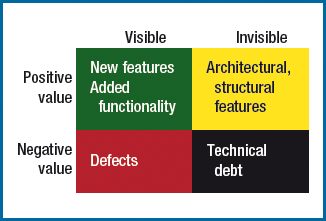
\includegraphics[width=0.8\textwidth]{images/fourColorBacklog.png}
	\caption{The colors reconcile four types of possible improvements.}
	\label{fig:fourColorBacklog}
\end{figure}

SonarQube is an open source application for quality management. It manages results of various code analysis tools, and is used to analyze and measure a projects technical quality. The technical debt is computed based on the SQALE (Software Quality Assessment based on Lifecycle Expectations) methodology. SQALE is a method for assessing technical debt in a project. It is based on tools that analyze the source code of the project, looking at different types of errors such as mismatched indentation, and different naming conventions. Each error is assigned a score based on how much work it would take to fix that error. The analysis gives a total sum of technical debt for the entire project.



%\subsection{Organizational debt}
%While technical debt is known problem, there's one more type of debt which can be accrued on a compandy-wide level. This type of debt is called organizational debt. Organizational debt is all about people and culture compromises made to \textit{'just get it done'} in early stages of a startup, preventing a company from running smoothly\cite{steve-blank}. When things should be going great, organizational debt can turn a growing company to a nightmare. Growing companies needs to know how to recognize and refactor organizational debt. 

%Some of the causes behind organizational debt might be:

%\begin{itemize}
%	\item Training the new hires, both culture and specific tasks
%	\item Retain existing hire by doing something for them. Many doesn't get promoted. New hire might get a better posistion than existing hire who has been there from the start.
%\end{itemize}

%Sometimes, the employees gets awarded by good building, new furnitures, and compensation for executive staff. However, that isn't enough. Think about existing employees who's been there from the start. You might end up loosing qualified people who's spent years building up the company, but not compensated for it. Top-down approach is focused too much. Think about the bottom employees.They have the inistituinal knowledge and hard-earned skills.

%When new people got hired, the ones who could train them about the company culture and how to do their specific tasks is the old employees who's being underpaid. They will look for another job. No one would be able to train the new people then. Giving compensation in form of stock vesting, insurance benefits, movie nights etc isnt enough as everyone gets it. Do something for the employees who's been there for a long time.

%Refarocting might be important in order to reduce the organizational debt. Write plan for managing new wave of hires before hiring them. Sometimes, you'll also need to think about what you will have to do if you're about to loose a key employee. Is it worth to replace employees who hold critical knowledge? Put together an expence budget using the current employee salaries. See who's important. Identify the one they wanted to keep and upgrade them. Some employees might not be that important as welll as they might be a performance problem for the whole organization. Need to look at the company culture as well, does it take into account of the new size and stage of the organization? What have the company achieved, what are the key elements that have made it great so farm, are they same of different. Think about the customer too. Does we talk to the customer, or does the customer talk to us. Also, keep in mind that an adivosory board of other CEOS who've been through the early stages might be good. Failure to refactor might kill a growing company\cite{steve-blank}.

%Some examples on organizational debt:
%\begin{itemize}
%	\item Different departments solving the same problems might use differnet methologies and tools. Difficult to see similarities in order to address company-wide issues.
%	\item Creation of processes and implement solutions which seems great at first, but didnt address the root casue of the issue and ending up creating more problems.
%	\item Time constraints, solving a problem in less-than-ideal manner this time. This manner is repeated because no one remember that the first time was intended to be one-off situation.
%\end{itemize}

%%%%%%%%%%%%%%%%%%%%%%%%%%%%%%%%%%%%%%%%%%%%%%%%%%%%%%%%%%%%%%%%%%%%%%%%%%%%%%%%%%%%%%

			% SOFTWARE LIFECYCLE

%%%%%%%%%%%%%%%%%%%%%%%%%%%%%%%%%%%%%%%%%%%%%%%%%%%%%%%%%%%%%%%%%%%%%%%%%%%%%%%%%%%%%%

\section{Software Lifecycle}
A software lifecycle is the phases a software product goes through between its convenient and when its no longer available for use\cite{159431}. There are five general groups of related activities in the software lifecycle according to IEEE Standard for Developing Software Life Cycle Processes\cite{159431}. 

\begin{enumerate}
	\item The first group is project management. Every software lifecycle starts with the project initiation. Project planning, and project monitoring and control are two other, necessary activities withing this group for each project iteration. 
	\item The second group is of pre-development. This group consists of activities that needs to be performed before the software development phase. Concept exploration is a good example of such activity. 
	\item The third group is the development itself. It includes the activities that must be performed during the development.
	\item The fourth group is of post-development. It includes activities to be performed after development to enchance the software project. The retirement activity involves removal of the existing system from its active support by ceasing its operation or support, or replacing it with a new system or an upgraded version of the exisiting system. 
	\item The final group is called integral. This group consists of activities that are necessary to ensure successful completion of a project. These activities is seen as support activities rather than activities that are directly oriented to the development effort.
\end{enumerate}

\subsection{Software Development Life Cycle and Methodologies} % (fold)
A software development process or a software development lifecycle is defined as the process by which user needs are translated into a software product\cite{radatz1990ieee}. The process involves translating user needs into requirements, transforming requirements into design, implementing design into code, testing the code, and sometimes, installing and checking out the software for operational use.

A software development methodology is defined as a framework to structure, plan, and control the software development process. Many software development methodologies exists, and the basic lifecycle activities are included in all lifecycle models, often in different orders. The difference is in terms of time to release, risk management, and quality. The models can be of different types, but they are usually defined as traditional and agile software development methodologies.

\subsubsection{Traditional Software Development}
Traditional software development methodologies are based on a sequential series of steps. It usually starts with elicitation and documentation of a complete set of requirements, followed by architecture and high level design, development, testing, and deployment. The most well-known of these traditional software development methodologies is the Waterfall method, the oldest software development process model. The Waterfall Model divides the software development lifecycle into five distinct and linear stages\cite{Vliet:2008:SEP:1481475}; requirements engineering, design, implementation, testing, and maintenance. There are many risks associated with the use of Waterfall model\cite{hijazi2012review}:
\begin{itemize}
	\item \textbf{Continuous requirements change}: Requirements are specified at the beginning of the software development process, and the remaining software development activities have to follow the initial requirements. This kind of model is not appropiate to use for software where technology and business requirements always change. 
	\item \textbf{No overlapping between stages}: Each stage in the Waterfall model needs to be completed entirely before proceeding into the next phase.
	\item \textbf{Poor quality assurance}: Lack of quality assurance during the differnet phases is another source of risk. Testing the system is the last stage in the development prorcess. Thus, all problems, bugs, and risk are discovered too late.
	\item \textbf{Relatively long stages}: Long stages in the development process makes it difficult to estimate time and cost. Additionally, there is no working product until late in the development process. 
\end{itemize}

Using sequential design processes such as Waterfall model in software development processes to build complex, intensive systems is often a failure\cite{p50-allman}. According to the Standish Group, CHAOS Report of 2015 reveals that 29\% of all projects using Waterfall method tends to fail, with no useful software deployed. 

%This is why agile methods was made, where change and feedback is important. One of the benefits is the ability to quickly release new functionality. However, one of the problems with agile methods is that developers often wants to focus on implementing new fucntionality, which results in poor focus on design, code quality, testing, which again leads to technical debt.  

\subsubsection{Agile Methods}
To address the challenges posed by traditional methods, agile methods were developed as a set of lightweight methods\cite{hijazi2012review}. Agile methods try to deal with collaboration in a way that promotes adaptive planning, early delivery, and continuous improvement, making the development phase faster and more flexible regarding changes\cite{abrahamsson2002agile}. Agile Manifesto describes four values that defines agile software development\cite{agilemanifesto}: 
\begin{itemize}
	\item Individuals and interactions over processes and tools
	\item Working software over comprehensive documentation
	\item Customer collaboration over contract negotiation
	\item Responding to change over following a plan
\end{itemize}

\textbf{Scrum} is one of the most popular agile software development methodologies. It is an iterative and incremental software development model. An advantage with iterative procedures is that parts of a system is developed early on, and can be tested before implementation of other parts. This reduces the risk of having long stages. The idea with Scrum is to divide the development into short periods, called sprints. Unlike the approach in the Waterfall model, the team can estimate how long it will take to implement tasks which can be accomplished during each sprint. To implement the requirements step by step, a product backlog is kept containing the features that have yet to be implemented. The product backlog is not static as it changes to the needs of the project, with new features being added, and obsolete ones being removed. Sprint backlog is items from the backlog that a team works on during a sprint.

\textbf{Lean Development} adapts the concepts and principles of Toyota Product Development System, to the practice of developing software\cite{Poppendieck:2007:LSD:1248821.1248986}. It is seen as a key component in building a change tolerant business\cite{cawley2010lean}. The seven lean principles that is applied to software development can be summarized as \textit{eliminate waste, build quality in, create knowledge, defer commitment, deliver fast, respect people, and optimize the whole}\cite{Pressman:2009:SEP:1593949,Poppendieck:2007:LSD:1248821.1248986}. These principles has many similarities with the Agile Manifesto.

Moreover, there are many risks associated with agile methodologies\cite{hijazi2012review}:
\begin{itemize}
	\item \textbf{Very large software system}: Developing large, complex software systems results in large increments. This increase the time span between increments, and thus require a higher cost to deal with changes and bugs if discovered.
	\item \textbf{Large development team}: Having large teams results in difficulities in managing communication between team members.
	\item \textbf{High reliance on human factor}: Agile methodologies relies on the development team, and their abilities to communicate with the customers.
	\item \textbf{Inappropriate customer representative}: This factor can influence the development process and the team members.
	\item \textbf{Distributed development environment}: Agile methodologies requires close interaction between the development team. Having a distributed development environment might challenge the communication between team members due to different time zones.
	\item \textbf{Scope creep}: With minimal planning conducted, developers can be easily distracted from the project main objectives.
\end{itemize}


\begin{figure}
	\centering
	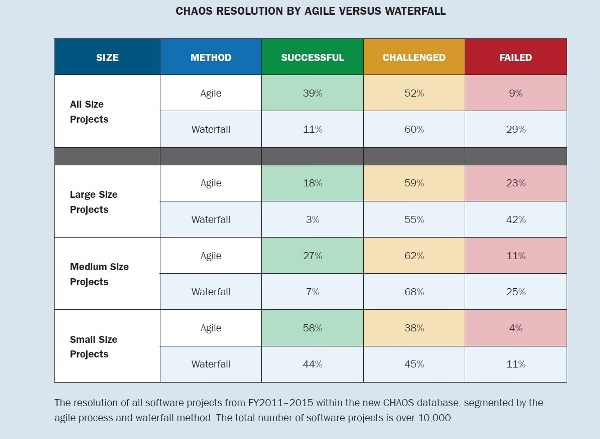
\includegraphics[width=0.8\textwidth]{images/Agile-Waterfall-Success-Failure-Rates.jpg}
	\caption{Agile implementation success rate by The Standish Group (SITER)}
	\label{fig:agileWaterfallSuccessFailureRates}
\end{figure}


%%%%%%%%%%%%%%%%%%%%%%%%%%%%%%%%%%%%%%%%%%%%%%%%%%%%%%%%%%%%%%%%%%%%%%%%%%%%%%%%%%%%%%

			% SOFTWARE ARCHITECTURE

%%%%%%%%%%%%%%%%%%%%%%%%%%%%%%%%%%%%%%%%%%%%%%%%%%%%%%%%%%%%%%%%%%%%%%%%%%%%%%%%%%%%%%
\section{Software Architecture}
Bass, Klements and Kazman\cite{Bass:2012:SAP:2392670} defines software architecture as following: 

\begin{displayquote}
The software architecture of a system is the set of structures needed to reason about the system, which compromise software elements, relations among them, and properties of both.
\end{displayquote}

The architecture of a software is one of the most important artifacts within the systems life cycle\cite{Bass:2012:SAP:2392670,knodel2006static}. Architectural design decisions that are made during the design phase, affect the systems ability to accept changes and to adapt to changing market requirements in the future. As the design decisions are made early, it will directly affect the evolution and maintenance phase\cite{Pressman:2009:SEP:1593949}, activities that consumes a big part of the systems lifespan\cite{Vliet:2008:SEP:1481475}. The problem of software architecture has long been a concern for those building and evolving large software systems\cite{perry1997state}.

Software architecture can be seen from two standpoints; prescriptive and descriptive architecture. The prescriptive architecture of a system captures the design decisions made prior to the construction. This is normally called as-conceived software architecture. Descriptive architecture describes how the system has actually been build, called for as-implemented software architecture. 

As the system evolves, it is ideal that the prescriptive architecture is modified first. In practice, the system - the descriptive architecture - is often directly modified. This can be due to developers sloppiness, short deadlines, or lack of documented prescriptive architecture. These principles introduces two new concepts; architectural drift and architectural erosion\cite{Bass:2012:SAP:2392670}. Architectural drift occurs when the documents are updated according to the implementation. The software architecture ends up as an architecture without vision and direction. Architectural erosion occurs when the implementation drifts away from the planned architecture. 

Long-term responsiveness of a system can be achieved by providing a solution of a system that would achieve certain quality attributes. The achievement of such quality attributes is based on the software architecure. 


%%%%%%%%%%%%%%%%%%%%%%%%%%%%%%%%%%%%%%%%%%%%%%%%%%%%%%%%%%%%%%%%%%%%%%%%%%%%%%%%%%%%%%

		% SOFTWARE MAINTENANCE AND EVOLUTION

%%%%%%%%%%%%%%%%%%%%%%%%%%%%%%%%%%%%%%%%%%%%%%%%%%%%%%%%%%%%%%%%%%%%%%%%%%%%%%%%%%%%%%
\section{Software Evolution}
Increasingly, more and more software developers are employed to maintain and evolve existing systems instead of developing new systems from scratch\cite{Sommerville:2011:SE}. Software evolution is a process that usually takes place when the initial development of a software project is done and was successful\cite{Bennett:2000:SME:336512.336534}. The goal of software evolution is to incorporate new user requirements in the application and adapt it to the existing application. Software evolution is important because it takes up to 85-90\% of organizational software costs\cite{Sommerville:2011:SE}. It is also important because technology tend to change rapidly, and not following these trend means loosing business oppertunities.

Rajlich and Bennet\cite{Bennett:2000:SME:336512.336534} proposed a view of the software lifespan, as shown in Figure \ref{fig:lifespan-1}. This view divides the software lifespan into five stages with initial development as the first stage. The key contribution is to seperate the maintenance phase into an evolution stage, followed by a service stage, and at last the phase-out stage.
\begin{description}
	\item[Initial development] produces the first version of the software from scratch.
	\item[Evolution] is the phase where significant changes to the software may be made. This could be addition of new features, correct previous mistakes, or adjust the software to new business requirements or technologies. Each change introduces a new feature or some other new property into the software.
	\item[Servicing] is the stage where relatively small, essential changes are allowed. The company considers how the software can be replaced. Legacy software is a term to describe software in this stage.
	\item[Phase-out] is the phase where software may still be used, but no further changes are being implemented. Users must work around any problems that they discover, or replace the software with something else.
	\item[Close-down] is when the managers or customers completely withdraw the system from production.
\end{description} 

\begin{figure}[ht!]
	\centering
	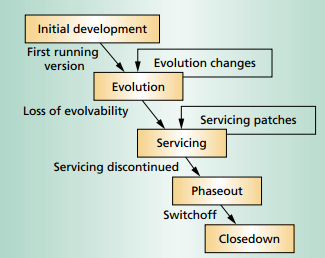
\includegraphics[width=0.8\textwidth]{images/lifespan-1.png}
	\caption{Software evolution process}
	\label{fig:lifespan-1}
\end{figure}

A variation of this process is the versioned stage model, as shown in Figure \ref{fig:lifespan-2}. When a software version is completed and released to the customer, the evolution continues with the company eventually releasing another version and only servicing the previous version. 

\begin{figure}[ht!]
	\centering
	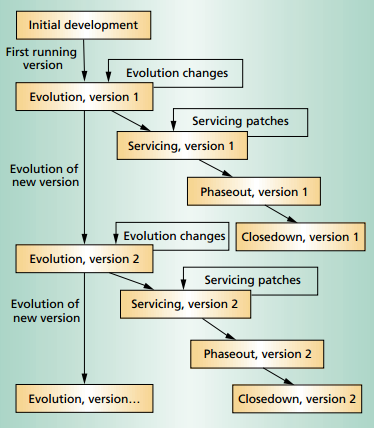
\includegraphics[width=0.8\textwidth]{images/lifespan-2.png}
	\caption{Software lifespan}
	\label{fig:lifespan-2}
\end{figure}

\subsection{Evolution Processes}
Software evolution usually starts with change proposals, which may be new requirements, existing requirements that have not been implemented, or bug reports from stakeholders. The process of implementing a change goes through these stages\cite{Sommerville:2011:SE} as shown in Figure \ref{fig:seProcess}.

The process starts with a set of proposed change requests. The cost and impact of the change is analyzed to decide whether to accept or deny the proposed changes. If the proposed changes are accepted, a new release of the system is planned. During release planning, all proposed changes such as fault repair, adaptation, and new functionality, are considered, to decide which changes to implement in the next version of the system. The changes are implemented and validated, and a new version of the system is released. The process ends with a new iteration with a set of proposed change requests for the next release. 

Sometimes, the need ofurgent changes may appear, such as a serious system fault that must be repaired to allow normal operation. In these cases, the usual process will not be beneficial as it takes time. An emergency fix is usually made to solve the problem. A developer choose a quick and workable solution rather than the best solution. The trade-off is that the the requirements, the software design, and the code become inconsistent. As a system changes over time, it will have impact on the systems internal structure and complexity. Software evolution might cause poor software quality and erosion of software architecture over time\cite{Bass:2012:SAP:2392670}.

\begin{figure}[h!]
	\centering
	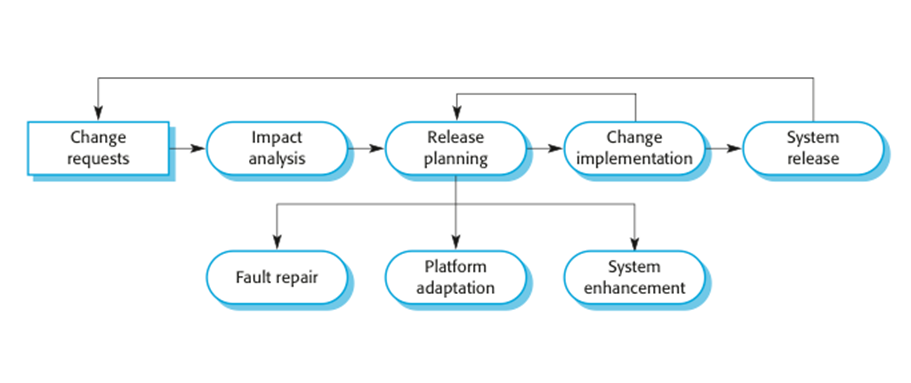
\includegraphics[width=0.8\textwidth]{images/SEprocess.png}
	\caption{Software evolution process}
	\label{fig:seProcess}
\end{figure}


\subsection{Software Maintenance}
IEEE 1219 defines software maintenance as follows\cite{720567}:
\begin{displayquote}
Modification of a software after delivery to correct faults, to improve performance or other attributes, or to adapt the product to a modified environment.
\end{displayquote} 
Maintenance can be classified into four types\cite{Bennett:2000:SME:336512.336534,720567}.

\begin{itemize}
	\item Adaptive: Modification of a software product performed after delivery to keep a computer program usable in a changed or changing environment.
	\item Perfective: Modification of a software product after delivery to improve performance or maintainability.
	\item Corrective: Reactive modification of a software product performed after delivery to correct discovered faults.
	\item Preventive: Maintenance performed for the purpose of preventing problems before they occur.
\end{itemize}

According to van Vliet, the real maintenance activity is corrective maintenance\cite{Vliet:2008:SEP:1481475}. 50\% of the total software maintenance is spent on perfective, 25\% on adaptive maintenance, and 4\% on preventive maintenance. This leads to that 21\% of the total maintenance activity is corrective maintenance, the 'real' maintenance\cite{Vliet:2008:SEP:1481475}. This has not changed since the 1980s when Lientz and and Swanson conducted a study on software maintenance\cite{lientz1980software}. Their study found out that most severe maintenance problems were caused by poor documentation, demand from users for changes, poor meeting schedulment, and problems training new hires. Some other problem areas were lack of user understanding, user training, and that customers did not understand how the system worked.

\begin{figure}
	\centering
	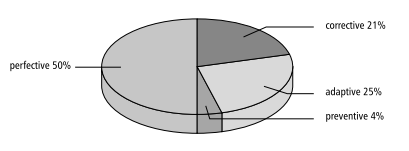
\includegraphics[width=0.8\textwidth]{images/maintenance.png}
	\caption{Distribution of maintenance activities\cite{Vliet:2008:SEP:1481475}}
	\label{fig:maintenanceActivities}
\end{figure}



%%%%%%%%%%%%%%%%%%%%%%%%%%%%%%%%%%%%%%%%%%%%%%%%%%%%%%%%%%%%%%%%%%%%%%%%%%%%%%%%%%%%%%

			% SOFTWARE REUSE

%%%%%%%%%%%%%%%%%%%%%%%%%%%%%%%%%%%%%%%%%%%%%%%%%%%%%%%%%%%%%%%%%%%%%%%%%%%%%%%%%%%%%%
\section{Software Reuse}
Software reuse is the process of using existing software artifacts, or knowledge, to create new software, rather than building it from scratch. Software reuse is a key method for improving software quality\cite{frakes1996software}. Software reuse can be specified in two directions, development \textit{for} reuse, and development \textit{with} reuse\cite{Slyngstad:2006:ESD:1159733.1159770}. Development for reuse is related to components for reuse or system generalization. Development with reuse is related to how existing components can be reused in new system.

Table \ref{tab:reusableComponents} lists several assets from a software project that can be reused\cite{frakes1996software}.
\begin{table}[H]
	\centering
	\begin{tabular}{ | l | l |}
	\hline
	1. architectures & 6. estimates \\ \hline
	2. source code & 7. human interfaces \\ \hline
	3. data & 8. plans \\ \hline
	4. designs & 9. requirements \\ \hline
	5. documentation & 10. test cases \\
	\hline
	\end{tabular}
	\caption{Reusable assets in software projects} \label{tab:reusableComponents}
\end{table}

Slyngstad et al.\cite{Slyngstad:2006:ESD:1159733.1159770} conducted an empirical study in Statoil ASA where their goal was to characterize developers views on software reuse. The results showed that reuse include lower costs, shorter development time, higher quality of the reusable components, and a standardized architecture. These findings are very similar to the key benefits of reuse that Lim has described\cite{lim1994effects}. The quality of software artifacts increases everytime the item is reused, because errors are discovered more frequently, making it easier to keep the artifact more stable\cite{sametinger1997software}.

Additionally, there can be problems associated with software reuse. A case study on a selected feature from self-driving miniature car development revealed that reuse of legacy, third party, or open source code, was one of the root causes for the accumulation of technical debt\cite{6974884}. Morisio et al.\cite{995420} idenfitied three main causes of software reuse failure; not introducing reuse-specific processes, not modifying nonreuse processes, and not considering human factors, combined with lack of commitment by top management.

%%%%%%%%%%%%%%%%%%%%%%%%%%%%%%%%%%%%%%%%%%%%%%%%%%%%%%%%%%%%%%%%%%%%%%%%%%%%%%%%%%%%%%

			% REFACTORING

%%%%%%%%%%%%%%%%%%%%%%%%%%%%%%%%%%%%%%%%%%%%%%%%%%%%%%%%%%%%%%%%%%%%%%%%%%%%%%%%%%%%%%
\section{Refactoring}
Design debt, a specific type of technical debt, accumulates as you write code\cite{Zazworka:2011:PDD:1985362.1985372}. This type of debt can be reduced when you refactor. Fowler defines refactoring as means of adjusting the design and architecture towards new requirements without changing the externial behaviour of a program in order to improve the quality of the system\cite{1999:RID:311424}. It is an act of improving the design of an existing system\cite{Vliet:2008:SEP:1481475}. Most of the time in spent on reducing design debt is on refactoring activities itself. These activities includes planning the design and architecture, rewriting the code, and adjusting documentation\cite{Pressman:2009:SEP:1593949}. It is believed that refactoring improves software quality and developer productivity, by making it easier to understand and maintain software codes\cite{Kim:2012:FSR:2393596.2393655}, thus a way to manage the technical debt of a system. 

Table \ref{tab:refactorArtifacts} lists the software artifacts that can be refactored\cite{1265817}.

\begin{table}[ht!]
	\renewcommand{\arraystretch}{1.2}
	\centering	
	\begin{tabular}{p{0.6\textwidth}} \hline
		\textbf{Programs} \\Refactoring at the source code or program level. For example, extracting methods, and encapsulating fields. \\ \hline
		\textbf{Designs} \\
		Refactoring at design level, for example in the form of UML models. Design patterns, software architecture, and database schemas, are some examples on artifacts that can be refactored at this level. \\ \hline
		\textbf{Software Requirements} \\
		Refactoring at the level of requiremetns specification. For example, decomposing requirements into a structure of viewpoints. \\ \hline
	\end{tabular}
	\caption{Types of Software Artifacts that can be refactored.}
	\label{tab:refactorArtifacts}
\end{table}


%%%%%%%%%%%%%%%%%%%%%%%%%%%%%%%%%%%%%%%%%%%%%%%%%%%%%%%%%%%%%%%%%%%%%%%%%%%%%%%%%%%%%%

			% CONFIGURATION MANAGEMENT

%%%%%%%%%%%%%%%%%%%%%%%%%%%%%%%%%%%%%%%%%%%%%%%%%%%%%%%%%%%%%%%%%%%%%%%%%%%%%%%%%%%%%%
\section{Configuration Management}
Systems always change to cope with bugs and introduce new features. A new version of a system is created when changes are made. Dart\cite{dart1991concepts} defines configuration management (CM) as a dicipline for controlling the evolution of software systems. CM identifies every component in a project and has an overview of every suggestions and changes from day one to the end of the product. CM involves four related activities\cite{Sommerville:2011:SE}:
\begin{description}
	\item[Change management] is intented to ensure that the evolution of a system is a managed process, and to prioritize changes. Costs and benefits has to be analyzed to approve changes and trach what components have been changed. The process starts with an actor submitting a change request. The request is checked for validity. If it is valid, the costs to this change are analyzed. The change request is passed to the change control board if it is not minor. The impact of the change from a strategic and organizational standpoint is considered, and if it is accepted, it is passed on. There are some important factors in the decision making process\cite{Sommerville:2011:SE}:\\
	\begin{inparaenum}[\itshape a\upshape)]
		\item The consequences of not making the change
		\item The benefits of the change
		\item The number of users affected by the change
		\item The costs of making the change
		\item The product release cycle
	\end{inparaenum}
	\item[Version management] is the process of keeping track of different and multiple versions of system components and ensuring that changes made to compoentns by different developers do not interfere with each other. This is often done with version management tools, which provide features like\\
	\begin{inparaenum}[\itshape a\upshape)]
		\item version and release identification;
		\item storage management;
		\item change history recording;
		\item independent development; or
		\item project support
	\end{inparaenum}
	\item[System building] creates an executable system by compiling and linking the program components, data, and libraries. The build process involves checking out component versions from the repository managed by the version management system, so it is necessary for system build tools and version management tools to communicate. There are many system build tools available, which provides features like 
	\begin{inparaenum}[\itshape a\upshape)]
		\item build script generation;
		\item version management system integration;
		\item executable system creation;
		\item test automation; or
		\item document generation.
	\end{inparaenum}
	\item[Release management] prepares the software for external release and keeps track of the system versions that have been released for customer use. Managing releases is a complex process as a release needs documentation such as configuration files, data files, and an installation program. Some factors that influences release planning are
	\begin{inparaenum}[\itshape a\upshape)]
		\item the technical quality of the system;
		\item platform changes;
		\item Lehman's fifth law;
		\item competitions;
		\item market requirements; or
		\item customer change proposals.
	\end{inparaenum}
\end{description}

There are some challenges related to development of embedded systems\cite{Estublier:2000:SCM:336512.336576}:
\begin{itemize}
	\item \textbf{Complex file sets}: Embedded systems consists of multiple diverse components, both hardware and software. This makes the system complex. Embedded system may also have different adjustable compoents for a specific platform, makin it easier to sell a product by tweaking some parameters. Dealing with these variates is a major challenge. Another challenge is that a product requires correct version of a component. Ensuring the consistency between components and their dependens files is a challenge as well.
	\item \textbf{Distributed teams}: Components may be developed in different places in our worl. Two team might for example work on the same components, especially when development are being outsourced. Such collaboration needs every developer to access each others work. The challenge is keep the team syncronized. 
	\item \textbf{Management and versioning of intellectual property}: Embedded systems, or software generally might use third-party technologies. It is important that those technologies are up-to-date, and maintained. These updates needs to be tracable such that each components has the right, compatible and stable version of its software. If something is not outsourced, it might be a challenge for developers to contribute and trace their changes.
\end{itemize}

Software CM (SCM) is the task of tracking and controlling changes in the software through reliable version selection and version control. SCM is a part of CM. Some examples on SCM that is widely used is Git, SVN, and Adele. Choosing a robust SCM system makes it possible to deal with big and complex files. It also supports distributed development. The right combination of SCM system and best practices makes it possible for embedded development projects to progress fast and efficiently. 



%%%%%%%%%%%%%%%%%%%%

% Kvalitet

%%%%%%%%%%%%%%%%%%%%%

\section{Software Quality}
Software Quality (SQ) is defined as \textit{an effective software process applied in a manner that creates a useful product that provides measurable value for those who produce it and those who use it}\cite{Pressman:2009:SEP:1593949}. The international standard for the evaluation of software quality presents six general properties that aims to give an overview of the software quality: functionality, reliability, usability, efficiency, maintainability, and portability. Table \ref{tab:qattribute} summarizes each quality attribute:

\begin{table}[ht!]
	\centering
	\begin{tabular}{ | l | p{8cm} |}
	\hline
	\textbf{Attribute} & \textbf{Description} \\ \hline
	Functionality 		& Ability of the system to do work for which it was intended. \\ \hline
	Reliability 		& Ability of the system to keep operating over time under certain conditions. \\ \hline
	Usability 			& The capability of the software product to be understood, learned, and used by users. \\ \hline
	Efficiency 			& The capability of the software product to provide appropriate performance, relative to the amount of resources used, under stated conditions. \\ \hline
	Maintainability 	& The capability of the software product to be modified in the future.\\ \hline
	Portability 		& The capability of the software product to be transferred from one environment to another. \\ \hline
	\end{tabular}
	\caption{Software Quality Attributes} \label{tab:qattribute}
\end{table}



%%%%%%%%%%%%%%%%%%%%%%%%%%%%%%%%%%%%%%%%%%%%%%%%%%%%%%%%%%%%%%%%%%%%%%%%%%%%%%%%%%%%%%
			
				% EMBEDDED SYSTEMS %

%%%%%%%%%%%%%%%%%%%%%%%%%%%%%%%%%%%%%%%%%%%%%%%%%%%%%%%%%%%%%%%%%%%%%%%%%%%%%%%%%%%%%%
\section{Embedded Systems}
%https://www.quora.com/What-are-the-characteristics-of-embedded-system

\textit{IEEE Standard Glossary of Software Engineering Terminology}\cite{radatz1990ieee} defines an embedded system as:
\begin{displayquote}
	\textit{A computer system that is part of a larger system and performs some of the requirements of that system; for example, a computer system used in an aircraft or rapid transit system.}
\end{displayquote}

While traditional computers are designed for performing multiple tasks, embedded systems are designed to perform a specific task under certain constraints. Embedded systems consists of small parts within a larger device that serves a more general purpose. For example, an embedded system in an automobile provides specific functions as a subsystem for the car itself\cite{Crnkovic:2005:CSE:1062455.1062631}. Due to their operational environment characteristics and common requirements, embedded systems are known as safety-critical and real-time systems\cite{563572,Crnkovic:2005:CSE:1062455.1062631}. This means that properties such as response time and worst case execution time are important design concerns\cite{4519555}: \textit{When the break pedal is pressed, the computer should initiate the breaking action within one millisecond}. A study of embedded systems shows that the various types of embedded systems share common requirements such as: \textit{real-time requirements, resource consumption, dependability, and life-cycle properties}\cite{crnkovic2004component}. It is expected that embedded systems are failure-free\cite{you2013reliability}, but these requirements might hinder embedded systems to deliver reliable service given a disturbance to its services, for example, failure in components\cite{patil2009embedded}. Additionally, it is expected that embedded systems has long life time\cite{563572}. Embedded systems are usually developed to deliver a service for long periods of time. Many of the embedded systems today were made many years ago, and thus have many weaknesses. 

Embedded software is defined as a computer software for embedded systems\cite{radatz1990ieee}. It includes the programs necessary to give functionality to the system hardware. As it runs on specialized type of hardware, embedded software has multiple contstrains related to run-time, memory usage, and processing power. Additionally, some other issues that needs to be addressed includes unstable requirements, technology changes, location of software errors, and inadequate documentation\cite{jimenez2013introduction}. In most cases, embedded software developers face many challenges in their work like conflicts in the requirements placed on them, for example, low memory usage while ensuring high availability\cite{vulgarakis2008embedded}. Moreover, old software are usually hard to maintain compared to new one, as they were made many years ago. Since embedded software has hardware constraints, companies must maintain many different configurations which makes maintenance a time challenge. Managing software quality is therefore necessary to deliver software in a useful, safe, and reliable way\cite{563572}. 





%Maintainability in embedded systems is as a property that allows the system to be acted upon, to guarantee a reliable operation thoroughout the end of its useful life\cite{introduction to embedded systems boka}. This property can be seen as a design constraint because it has to be planned from the project initiation. Large, expensive, and complex embedded systems are expected to remain in operation for decades, thus making maintenance an important property which allows reliable operation.

There are several challenges designers faces when it comes to integrating maintainability in embedded software. To improve the maintainability of embedded systems, some issues needs to be adressed, which includse unstable requirements, technology changes, location of software errors, hardware constraints, and inadequate documentation. Research has shown that addressing some of these changes improves the maintainability of embedded systems.


\subsection{Security}
Sommerville defines security as \textit{a systems ability to resist attacks. It is a complex property that cannot be easily measured. Attacks may be devised that were not anticipated by the system designers and so may defeat built-in safeguards}\cite{Sommerville:2011:SE}.
ISO 9126


\subsection{Dependability}



